% main.tex
% Double-column paper draft on Muon-inspired matrix optimization.

\documentclass[sigconf,nonacm]{acmart}

\usepackage{amsmath}
\usepackage{amsfonts}
\usepackage{amsthm}
\usepackage{booktabs}
\usepackage{colortbl}
\usepackage{graphicx}
\usepackage{multirow}
\usepackage{hyperref}

\settopmatter{authorsperrow=2}
\newcommand{\vpara}[1]{\par\noindent\textbf{#1.}\ }
\definecolor{bestgreen}{RGB}{223,242,225}
\definecolor{warnred}{RGB}{252,229,225}
\newcommand{\bestcell}[1]{\cellcolor{bestgreen}{#1}}
\newcommand{\warncell}[1]{\cellcolor{warnred}{#1}}
\newtheorem{proposition}{Proposition}
\newtheorem{lemma}{Lemma}
\newtheorem{remark}{Remark}
\DeclareMathOperator{\rank}{rank}
\DeclareMathOperator{\diag}{diag}

\title{Spectral-Norm Steepest Descent and Matrix Preconditioning: A Mechanistic Study Inspired by Muon Optimizers}

\author{Gaorui Zhang}
\affiliation{%
  \institution{Zhejiang University}
  \city{Hangzhou}
  \country{China}}
\email{gaoruizhang@zju.edu.cn}

\begin{document}

\begin{abstract}
Matrix-valued parameters in deep networks invite two different optimization mechanisms: curvature preconditioning, which changes objective geometry, and update normalization, which changes step geometry. This course report separates the two on the matrix quadratic objective $f(W)=\frac{1}{2}\|AWB-C\|_F^2$. The exact Hessian is $BB^\top\otimes A^\top A$, so an ideal left--right preconditioner can flatten the objective spectrum. Muon-style updates do not implement this operation. Their matrix-sign step solves a spectral-norm constrained steepest-descent problem and normalizes the singular values of the update rather than approximating an inverse Hessian. We then analyze three mechanisms that determine whether this spectral direction becomes a usable optimizer step: decoupled weight decay, update-RMS alignment across matrix shapes, and Newton--Schulz approximation quality. Synthetic quadratic diagnostics confirm the objective-spectrum versus update-spectrum separation, while scale checks and finite Newton--Schulz experiments isolate the stability mechanisms. Small-scale Digits sanity checks show that these mechanisms remain visible in full-batch neural-network training. The main conclusion is mechanistic: Muon-style orthogonalization changes update geometry, and its practical behavior depends on scale control after the spectral direction has been chosen. Code is available at \url{https://github.com/Galaxy-Dawn/muon-optimization-course-report}.
\end{abstract}

\maketitle

\section{Introduction}
Matrix-valued parameters are common in modern neural networks, especially in linear layers and projection matrices. Matrix-aware optimizers exploit this structure in different ways. Adam and AdamW scale coordinates independently with first- and second-moment statistics \citep{kingma2014adam,loshchilov2019adamw}. K-FAC and Shampoo use approximate curvature factors to precondition matrix or tensor updates \citep{martens2015kfac,gupta2018shampoo}. These methods change the geometry of the objective. Muon-style optimizers instead replace a momentum matrix by its polar factor, normalizing the update by its singular values \citep{kellerjordan2024muon}. The two operations are easy to group together because both transform the raw gradient, but they target different objects.

Recent work has made this distinction more important. Muon fits the broader view of norm-rescaled steepest descent \citep{bernstein2024oldoptimizer}, and finite Newton--Schulz approximation has been analyzed as a way to compute the polar step efficiently \citep{kim2026convergence}. Other variants add curvature or adaptivity around the polar step, including Newton-Muon and Muon$^2$ \citep{du2026newtonmuon,liu2026muon2}. At the same time, large-scale training reports emphasize decoupled weight decay, update-RMS alignment, and related scale controls as practical ingredients \citep{liu2025moonlight,su2025muonchoice,su2025qkclip}. The resulting literature mixes three questions: what changes the objective spectrum, what changes the update spectrum, and what makes the final step stable. Treating these questions as one mechanism obscures what Muon-style orthogonalization actually contributes.

This report studies that separation directly. We use the matrix quadratic objective
\begin{equation}
  f(W)=\frac{1}{2}\|AWB-C\|_F^2,
\end{equation}
because its Hessian is exactly Kronecker structured and the ideal left--right preconditioner is available in closed form. This gives an oracle reference for curvature correction. We then compare that reference with the Muon matrix-sign step, which solves a spectral-norm constrained steepest-descent problem. Finally, we analyze the scale and approximation mechanisms that are applied after the spectral direction is chosen: decoupled weight decay, RMS alignment across matrix shapes, and Newton--Schulz approximation quality.

The report makes three contributions. First, it gives a closed-form comparison between objective-spectrum preconditioning and update-spectrum normalization on a matrix quadratic model. Second, it shows that the Muon matrix-sign step is a spectral-norm steepest-descent direction rather than an inverse-Hessian approximation. Third, it tests the resulting decomposition with controlled synthetic diagnostics and small-scale neural-network experiments. The synthetic results support the mechanism-level claims directly; the Digits runs check whether the same scale and approximation effects appear during training.

The rest of the paper develops these points in order. Section~2 expands the related work on diagonal adaptivity, matrix preconditioning, and Muon variants. Section~3 derives the theory behind the Kronecker Hessian, the matrix-sign step, and the stability mechanisms. Section~4 presents the diagnostics. Sections~5 and~6 discuss limitations and conclude.

\begin{figure*}[t]
    \centering
    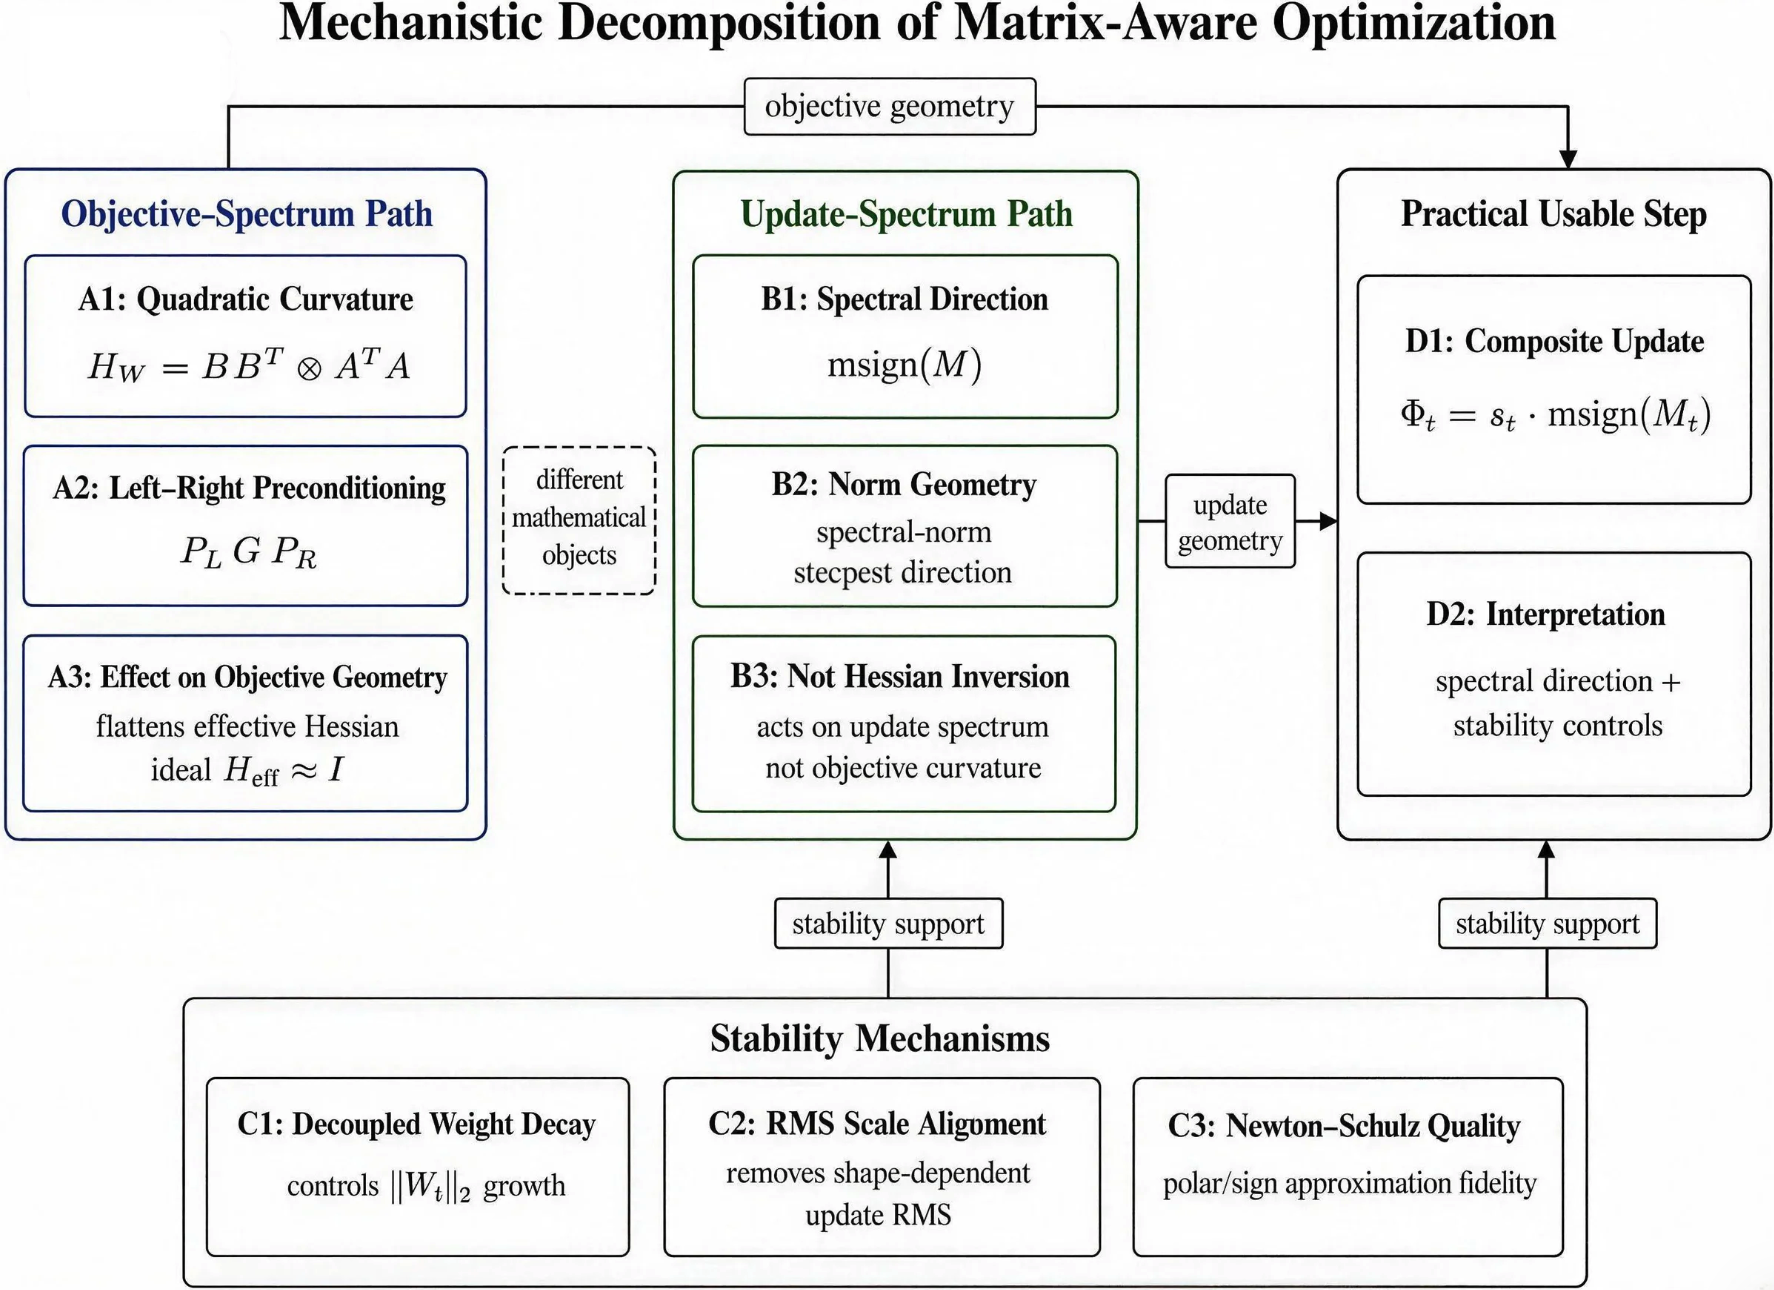
\includegraphics[width=0.70\textwidth]{figures/main_mechanism_user.png}
    \caption{Mechanistic decomposition of matrix-aware optimization. Objective-spectrum preconditioning targets curvature geometry, update-spectrum normalization via $\operatorname{msign}(\cdot)$ targets step geometry, and practical usable steps depend on three stability mechanisms: decoupled weight decay, RMS scale alignment, and Newton--Schulz approximation quality.}
    \Description{Closed block diagram separating objective-spectrum preconditioning, update-spectrum matrix-sign normalization, and stability mechanisms for practical matrix-aware optimization.}
    \label{fig:main_mechanism}
\end{figure*}

\section{Related Work}
\vpara{Diagonal adaptive methods} AdaGrad scales each coordinate by the accumulated magnitude of past gradients \citep{duchi2011adagrad}. Adam combines exponential moving averages of gradients and squared gradients, and AdamW decouples weight decay from the adaptive update \citep{kingma2014adam,loshchilov2019adamw}. These methods are computationally efficient, but their preconditioners are diagonal in the parameter basis. They correct coordinate-wise scale without modeling rotations of the local Hessian. Decoupled weight decay separates weight shrinkage from the update direction. This makes MuonW a contraction of the current matrix followed by a bounded spectral update. AdamW is both a baseline and a reference mechanism.

\vpara{Matrix preconditioning} K-FAC approximates the Fisher or Gauss--Newton matrix by Kronecker factors and inverts the factors separately \citep{martens2015kfac}. Shampoo maintains positive-definite preconditioners along tensor dimensions \citep{gupta2018shampoo}. These algorithms implement curvature correction by changing the metric in which the loss is optimized. The quadratic model $f(W)=\frac12\|AWB-C\|_F^2$ is exactly Kronecker structured, so the ideal preconditioner can be written in closed form. The model is an oracle reference for curvature correction. It also gives a direct comparison point for Muon-style steps.

\vpara{Norm-rescaled and orthogonalized updates} Bernstein and Newhouse view several optimizers as steepest descent under non-Euclidean update norms \citep{bernstein2024oldoptimizer}. Muon fits this perspective because it replaces a momentum matrix by its polar factor \citep{kellerjordan2024muon}. Kim and Oh analyze convergence when the polar factor is approximated by finitely many Newton--Schulz iterations \citep{kim2026convergence}. Newton--Muon adds an input-covariance right-preconditioner before the polar step \citep{du2026newtonmuon}. Muon$^2$ adds an Adam-like second-moment preconditioner before orthogonalization \citep{liu2026muon2}. Moonlight and related discussions emphasize decoupled weight decay and update-RMS alignment across parameter shapes as practical scale-up mechanisms \citep{liu2025moonlight,su2025muonchoice}. Later work identifies maximum-logit growth as another potential instability \citep{su2025qkclip}. The present paper does not reproduce large-scale language-model training. It isolates which aspects of Muon follow from linear algebra and which remain empirical scale-up considerations.

\section{Theory: Matrix Preconditioning and Spectral Updates}
This section establishes the theoretical basis of the paper. We first recall how condition numbers control gradient descent on vector quadratics, then derive the Kronecker Hessian of a matrix quadratic objective. We next show that Muon-style matrix-sign updates solve a spectral-norm steepest-descent problem. Finally, we analyze three stabilizing mechanisms: decoupled weight decay, RMS scale alignment, and Newton--Schulz approximation.

The analysis proceeds in stages. We first examine the behavior of an ideal matrix preconditioner under known curvature. We then show that the matrix sign solves a different constrained first-order problem. Finally, we add the scale and approximation mechanisms that convert the spectral direction into an optimizer step. The notation below separates these objects deliberately: $H_W$ denotes objective curvature, $G$ or $M_t$ denotes a gradient or momentum matrix, and $\Phi_t$ denotes the actual update direction after normalization or scaling.

We use two condition-number conventions. For $M\succ0$,
\begin{equation}
  \kappa(M)=\frac{\lambda_{\max}(M)}{\lambda_{\min}(M)}.
\end{equation}
For a full-rank rectangular matrix $A$,
\begin{equation}
  \kappa(A)=\frac{\sigma_{\max}(A)}{\sigma_{\min}(A)}.
\end{equation}
All vectorizations use the standard column-stacking convention, so that
\begin{equation}
  \operatorname{vec}(LXR)=(R^\top\otimes L)\operatorname{vec}(X)
\end{equation}
whenever the products are well defined.

\subsection{Quadratic objectives and matrix preconditioning}
\vpara{Vector quadratics} Consider
\begin{equation}
  f(x)=\frac{1}{2}(x-x^\star)^\top H(x-x^\star), \qquad H\succ 0.
\end{equation}
Let $e_t=x_t-x^\star$. Since $\nabla f(x_t)=He_t$, gradient descent gives $e_{t+1}=(I-\eta H)e_t$.

\begin{proposition}[Condition-number controlled convergence]\label{prop:gd}
Assume $H\succ0$ and let $0<\eta<2/\lambda_{\max}(H)$. Then gradient descent converges linearly in the Euclidean norm. Among constant step sizes, the minimizer of the worst-case Euclidean contraction factor
\begin{equation}
  \sup_{e\neq0}\frac{\|(I-\eta H)e\|_2}{\|e\|_2}
\end{equation}
is
\begin{equation}
  \eta^\star=\frac{2}{\lambda_{\max}(H)+\lambda_{\min}(H)},
\end{equation}
and it yields
\begin{equation}
  \|e_t\|_2 \leq \left(\frac{\kappa(H)-1}{\kappa(H)+1}\right)^t\|e_0\|_2 .
\end{equation}
For the preconditioned update $x_{t+1}=x_t-\eta P\nabla f(x_t)$, choosing $P=H^{-1}$ gives $e_{t+1}=(1-\eta)e_t$. Hence $\eta=1$ gives one-step convergence.
\end{proposition}

\begin{proof}
Let $H=Q\Lambda Q^\top$ with $\Lambda=\diag(\lambda_1,\ldots,\lambda_d)$ and $0<\lambda_{\min}\leq\lambda_i\leq\lambda_{\max}$. In the coordinates $y_t=Q^\top e_t$,
\begin{equation}
  y_{t+1}^{(i)}=(1-\eta\lambda_i)y_t^{(i)}.
\end{equation}
Since $I-\eta H$ is symmetric,
\begin{equation}
  \sup_{e\neq0}\frac{\|(I-\eta H)e\|_2}{\|e\|_2}
  =\|I-\eta H\|_2
  =\max_i|1-\eta\lambda_i|.
\end{equation}
Consequently
\begin{equation}
  \|e_t\|_2\leq \rho(\eta)^t\|e_0\|_2,\qquad
  \rho(\eta)=\max_i |1-\eta\lambda_i| .
\end{equation}
The condition $0<\eta<2/\lambda_{\max}$ implies $|1-\eta\lambda_i|<1$ for every $i$, so $\rho(\eta)<1$ and the convergence is linear. For fixed $\eta$, the scalar function $\lambda\mapsto |1-\eta\lambda|$ is convex on $[\lambda_{\min},\lambda_{\max}]$, so its maximum over this interval is attained at one of the two endpoints. Thus
\begin{equation}
  \rho(\eta)=\max\{ |1-\eta\lambda_{\min}|, |1-\eta\lambda_{\max}|\}.
\end{equation}
The minimax value is obtained by equalizing the two endpoint magnitudes,
\begin{equation}
  1-\eta\lambda_{\min}=\eta\lambda_{\max}-1,
\end{equation}
which gives $\eta^\star=2/(\lambda_{\max}+\lambda_{\min})$ and
\begin{equation}
  \rho(\eta^\star)=
  \frac{\lambda_{\max}-\lambda_{\min}}
       {\lambda_{\max}+\lambda_{\min}}
  =\frac{\kappa(H)-1}{\kappa(H)+1}.
\end{equation}
Finally, substituting $P=H^{-1}$ into $e_{t+1}=(I-\eta PH)e_t$ gives $e_{t+1}=(1-\eta)e_t$. See \citet{nocedal2006numerical} for the standard analysis.
\end{proof}

Large condition numbers degrade gradient-descent convergence. A successful curvature preconditioner makes the eigenvalues of the effective Hessian more uniform. This is the target of the matrix analysis below.

\vpara{Matrix quadratics} Let $W\in\mathbb{R}^{m\times n}$ and consider
\begin{equation}\label{eq:matrix_obj}
  f(W)=\frac{1}{2}\|AWB-C\|_F^2,
\end{equation}
where $A\in\mathbb{R}^{p\times m}$ has full column rank, $B\in\mathbb{R}^{n\times q}$ has full row rank, and $C=AW^\star B$ for some $W^\star$. Define $E_t=W_t-W^\star$.

\begin{proposition}[Kronecker Hessian]\label{prop:matrix_hessian}
For~\eqref{eq:matrix_obj}, the gradient is
\begin{equation}
  \nabla_W f(W)=A^\top(AWB-C)B^\top .
\end{equation}
In particular, along the realizable error $E_t=W_t-W^\star$,
\begin{equation}
  \nabla_W f(W_t)=A^\top A E_t BB^\top.
\end{equation}
With column-stacked vectorization, the Hessian is
\begin{equation}
  H_W=BB^\top\otimes A^\top A,
\end{equation}
and its condition number is $\kappa(H_W)=\kappa(A)^2\kappa(B)^2$.
\end{proposition}

\begin{proof}
Let $R(W)=AWB-C$. For any perturbation $\Delta$,
\begin{align}
  df(W)[\Delta]
  &=\left.\frac{d}{d\varepsilon}\frac12\|R(W)+\varepsilon A\Delta B\|_F^2\right|_{\varepsilon=0}\notag\\
  &=\langle R(W),A\Delta B\rangle_F \\
  &=\operatorname{tr}(R(W)^\top A\Delta B)\notag\\
  &=\operatorname{tr}((A^\top R(W)B^\top)^\top\Delta)\notag\\
  &=\langle A^\top R(W)B^\top,\Delta\rangle_F .
\end{align}
By the Riesz representation theorem for the Frobenius inner product, $\nabla_W f(W)=A^\top(AWB-C)B^\top$. If $C=AW^\star B$, then this becomes $A^\top A(W-W^\star)BB^\top$. Vectorizing the linear part and using the stated column-stacking identity gives
\begin{equation}
  \operatorname{vec}(A^\top A\,E\,BB^\top)
  =(BB^\top\otimes A^\top A)\operatorname{vec}(E).
\end{equation}
Since $A$ has full column rank and $B$ has full row rank, $A^\top A\succ0$ and $BB^\top\succ0$. The eigenvalues of a Kronecker product are pairwise products of the eigenvalues of the factors \citep{horn2012matrix}. Hence
\begin{equation}
  \kappa(H_W)=\kappa(A^\top A)\kappa(BB^\top)=\kappa(A)^2\kappa(B)^2.
\end{equation}
\end{proof}

\begin{lemma}[Injectivity and uniqueness of the realizable minimizer]\label{lem:injective}
Under the rank assumptions in~\eqref{eq:matrix_obj}, the linear map $\mathcal{T}(W)=AWB$ is injective. Consequently, if $C=AW^\star B$, then $W^\star$ is the unique global minimizer of $f$.
\end{lemma}

\begin{proof}
Suppose $AWB=0$. Since $A$ has full column rank, $A^\top A$ is invertible. Since $B$ has full row rank, $BB^\top$ is invertible. Therefore
\begin{equation}
  W=(A^\top A)^{-1}A^\top(AWB)B^\top(BB^\top)^{-1}=0.
\end{equation}
Thus $\ker\mathcal{T}=\{0\}$, so $\mathcal{T}$ is injective. In the realizable case, $f(W)\ge0$ and $f(W^\star)=0$. If $\widetilde W$ is any global minimizer, then $f(\widetilde W)=0$, hence $A(\widetilde W-W^\star)B=0$. Injectivity gives $\widetilde W=W^\star$.
\end{proof}

Lemma~\ref{lem:injective} is used in the experiments because $W^\star$ is identifiable in the realizable case $C=AW^\star B$. In that setting, both objective error and parameter error are unambiguous. In the non-realizable least-squares case the Hessian is the same, but the optimum generally has nonzero residual. We do not study that setting here. The Kronecker form also shows why a diagonal method can be insufficient. If the singular vectors of $A$ or $B$ are rotated relative to the coordinate axes, the Hessian in vectorized coordinates contains couplings that cannot be removed by scaling coordinates independently.

\vpara{Left--right preconditioning} The matrix objective admits an ideal left--right preconditioner.

\begin{proposition}[Ideal left--right preconditioning]\label{prop:lr}
Set $P_L=(A^\top A)^{-1}$ and $P_R=(BB^\top)^{-1}$. The update
\begin{equation}
  W_{t+1}=W_t-\eta P_L\nabla_W f(W_t)P_R
\end{equation}
satisfies
\begin{equation}
  E_{t+1}=(1-\eta)E_t.
\end{equation}
Thus $\eta=1$ gives one-step convergence.
\end{proposition}

\begin{proof}
Substitute Proposition~\ref{prop:matrix_hessian} into the update:
\begin{align}
E_{t+1}
&=E_t-\eta(A^\top A)^{-1}(A^\top A E_t BB^\top)(BB^\top)^{-1}\\
&=(1-\eta)E_t .
\end{align}
\end{proof}

Proposition~\ref{prop:lr} shows that ideal matrix preconditioning acts on the objective spectrum: in vectorized form, $(P_R^\top\otimes P_L)(BB^\top\otimes A^\top A)=I\otimes I$. Equivalently, it turns the effective Hessian of the quadratic into the identity. This gives a stringent benchmark against which spectral updates can be compared: in neural networks generally neither $A^\top A$ nor $BB^\top$ is known exactly, and the local curvature changes during training. The result is a mathematical reference, not a practical optimization method.

\subsection{Matrix-sign updates as spectral-norm steepest descent}
For a rank-$r$ matrix $G\in\mathbb{R}^{m\times n}$, write its compact SVD as $G=U_r\Sigma_rV_r^\top$. Define $\operatorname{msign}(G)=U_rV_r^\top$.

\begin{proposition}[Spectral-norm steepest descent]\label{prop:msign}
Let $G\in\mathbb{R}^{m\times n}$ be nonzero with compact SVD $G=U_r\Sigma_rV_r^\top$, and let $\eta>0$. Then one solution of
\begin{equation}
  \min_{\|\Delta W\|_2\leq \eta}\langle G,\Delta W\rangle_F
\end{equation}
is
\begin{equation}
  \Delta W^\star=-\eta U_rV_r^\top=-\eta\operatorname{msign}(G).
\end{equation}
If $r=\min(m,n)$, this minimizer is unique. If $r<\min(m,n)$, the minimizer is generally nonunique. Its normalized maximizer form is
\begin{equation}\label{eq:msign_solution_set}
  \Phi=U_rV_r^\top+Z,
  \qquad U_r^\top Z=0,\quad ZV_r=0,\quad \|Z\|_2\leq1,
\end{equation}
with $\Delta W^\star=-\eta\Phi$. If $G=0$, every feasible $\Delta W$ has the same first-order objective value. In implementations we set $\operatorname{msign}(0)=0$.
\end{proposition}

\begin{proof}
Write $\Delta W=-\eta\Phi$ with $\|\Phi\|_2\leq1$. The problem is equivalent to maximizing $\langle G,\Phi\rangle_F$ over the spectral-norm unit ball. By duality between the nuclear norm and the spectral norm,
\begin{equation}
  \langle G,\Phi\rangle_F\leq \|G\|_*\|\Phi\|_2\leq\|G\|_*.
\end{equation}
Equivalently, the first inequality follows from von Neumann's trace inequality \citep{horn2012matrix}. The choice $\Phi_0=U_rV_r^\top$ is feasible because $\|U_rV_r^\top\|_2=1$, and it attains equality:
\begin{equation}
  \langle G,U_rV_r^\top\rangle_F
  =\operatorname{tr}(V_r\Sigma_rU_r^\top U_rV_r^\top)
  =\operatorname{tr}(\Sigma_r)=\|G\|_*.
\end{equation}
Thus $-\eta U_rV_r^\top$ is a minimizer.

It remains to justify the uniqueness statement. Equality in the duality bound means that $\Phi$ lies in the subdifferential of the nuclear norm at $G$. For $G=U_r\Sigma_rV_r^\top$, this subdifferential is
\begin{equation}
  \partial\|G\|_*=
  \left\{U_rV_r^\top+Z:
  U_r^\top Z=0,\ ZV_r=0,\ \|Z\|_2\leq1\right\}.
\end{equation}
Hence all maximizers have the form~\eqref{eq:msign_solution_set}. If $r=\min(m,n)$, then either $U_r$ spans all of $\mathbb{R}^m$ or $V_r$ spans all of $\mathbb{R}^n$. The orthogonality constraints force $Z=0$. If $r<\min(m,n)$, nonzero matrices $Z$ satisfying the two orthogonality constraints exist, so the minimizer is generally nonunique.
\end{proof}

This result characterizes the direction of a Muon update, but it does not determine the scale or stability properties of the resulting optimizer. The result applies to the linear form induced by the current gradient or momentum matrix. When applied to a momentum matrix $M_t$, the direction $-\operatorname{msign}(M_t)$ is steepest for the momentum-defined surrogate linear objective $\langle M_t,\Delta W\rangle_F$, not necessarily for the instantaneous loss linearization $\langle G_t,\Delta W\rangle_F$. The polar factor preserves singular vectors and discards singular values. It is therefore not a Hessian inverse, and it does not replace $H_W$ by a better-conditioned effective Hessian. This also explains a phenomenon observed in the matrix-quadratic experiment. Even on an isotropic objective, the matrix sign may converge slowly if the error matrix has a highly nonuniform singular-value profile. Gradient descent follows the singular values of the error, while $\operatorname{msign}$ discards them.

\subsection{Decoupled weight decay and spectral-norm control}
Practical Muon variants commonly combine the polar direction with decoupled weight decay, in analogy with AdamW. Let
\begin{equation}
  W_{t+1}=(1-\eta\lambda)W_t-\eta\Phi_t,
\end{equation}
where $\Phi_t$ denotes the full direction before multiplication by $\eta$. It may denote the unscaled polar direction $\operatorname{msign}(M_t)$ or a scaled polar direction such as $s_t\operatorname{msign}(M_t)$.

\begin{proposition}[Spectral-norm control under decay]\label{prop:decay}
Assume $\lambda>0$, $0\leq \eta\lambda\leq1$, and $\|\Phi_t\|_2\leq S$ for all $t$. Then
\begin{equation}
  \|W_t\|_2\leq \max\left\{\|W_0\|_2,\frac{S}{\lambda}\right\}
\end{equation}
for all $t$.
\end{proposition}

\begin{proof}
Let $R=\max\{\|W_0\|_2,S/\lambda\}$. We prove by induction that $\|W_t\|_2\leq R$. The claim is true at $t=0$. If it holds at time $t$, then by the triangle inequality,
\begin{align}
\|W_{t+1}\|_2
&\leq (1-\eta\lambda)\|W_t\|_2+\eta\|\Phi_t\|_2\\
&\leq (1-\eta\lambda)R+\eta S.
\end{align}
Since $R\geq S/\lambda$, we have $S\leq\lambda R$. Therefore
\begin{equation}
(1-\eta\lambda)R+\eta S\leq (1-\eta\lambda)R+\eta\lambda R=R.
\end{equation}
This completes the induction.
\end{proof}

For unscaled Muon, one may take $S=1$ because
\begin{equation}
  \|\operatorname{msign}(M_t)\|_2\leq1,
\end{equation}
with equality whenever $M_t\neq0$. For scaled Muon,
$\Phi_t=s_t\operatorname{msign}(M_t)$, one may take
$S=\sup_t s_t$ if this quantity is finite. Bounded-spectral-norm updates and decoupled decay control weight growth. Without decay, bounded update directions can still accumulate into large weight matrices over many steps. With decay, the recurrence has a stable radius proportional to the update spectral norm and inversely proportional to the decay coefficient. This bound controls weight growth, but it does not prove loss decrease or convergence to a minimizer. It motivates including AdamW and MuonW, rather than only Adam and decay-free Muon, in the Digits sanity checks.

\subsection{Update RMS alignment across matrix shapes}
The spectral norm controls the largest singular value, but the elementwise RMS of a matrix-sign update depends on the matrix shape. For $\Phi=\operatorname{msign}(M)$ with $M\in\mathbb{R}^{m\times n}$ and rank $r$,
\begin{equation}
  \|\Phi\|_F^2=r,
\end{equation}
since $\Phi$ has $r$ singular values equal to one.

\begin{proposition}[RMS of a matrix-sign update]\label{prop:rms}
Let $M\in\mathbb{R}^{m\times n}$ have rank $r$, and let $\Phi=\operatorname{msign}(M)$, with the convention $\operatorname{msign}(0)=0$. Define $\operatorname{RMS}(\Phi)=\|\Phi\|_F/\sqrt{mn}$. Then
\begin{equation}
  \operatorname{RMS}(\Phi)=\sqrt{\frac{r}{mn}}.
\end{equation}
If $M$ is full rank, then $\operatorname{RMS}(\Phi)=1/\sqrt{\max(m,n)}$.
\end{proposition}

\begin{proof}
If $r=0$, then $M=0$, $\Phi=0$, and the identity is immediate. Assume $r>0$ and let $M=U_r\Sigma_rV_r^\top$ be the compact SVD. Then $\Phi=U_rV_r^\top$. Since $U_r^\top U_r=I_r$ and $V_r^\top V_r=I_r$,
\begin{align}
\|\Phi\|_F^2
&=\operatorname{tr}(\Phi^\top\Phi)\\
&=\operatorname{tr}(V_rU_r^\top U_rV_r^\top)\\
&=\operatorname{tr}(V_rV_r^\top)\\
&=\operatorname{tr}(V_r^\top V_r)=r .
\end{align}
Dividing by $mn$ gives $\operatorname{RMS}(\Phi)=\sqrt{r/(mn)}$. If $M$ has full rank, then $r=\min(m,n)$, so $\sqrt{r/(mn)}=1/\sqrt{\max(m,n)}$.
\end{proof}

This proposition explains why Muon updates require shape-dependent scaling. Multiplying $\operatorname{msign}(M)$ by $\sqrt{\max(m,n)}$ makes the update RMS approximately one for full-rank matrices. This identity gives the algebraic basis for update-RMS alignment in scalable Muon implementations \citep{liu2025moonlight,su2025muonchoice}. A fixed learning rate can induce different elementwise step sizes across layers. A tall matrix and a square matrix have different raw matrix-sign RMS, even when both updates have unit spectral norm.

\subsection{Newton--Schulz approximation of the matrix sign}
Exact SVD-based computation of the matrix sign is expensive. Muon implementations approximate the polar factor through Newton--Schulz iterations. Consider the polynomial iteration
\begin{equation}\label{eq:ns}
  X_{k+1}=aX_k+bX_kX_k^\top X_k+cX_k(X_k^\top X_k)^2 .
\end{equation}

\begin{lemma}[Singular-value dynamics]\label{lem:ns}
Let $X_k\in\mathbb{R}^{m\times n}$ have compact SVD $X_k=U\Sigma_kV^\top$. Here
\[
\Sigma_k=\diag(\sigma_{1,k},\ldots,\sigma_{r,k})
\]
contains the positive singular values. Define
\begin{equation}
  p(s)=as+bs^3+cs^5 .
\end{equation}
Then the iteration~\eqref{eq:ns} satisfies
\begin{equation}
  X_{k+1}=U p(\Sigma_k)V^\top,
\end{equation}
where $p(\Sigma_k)=\diag(p(\sigma_{1,k}),\ldots,p(\sigma_{r,k}))$. Consequently, the nonzero singular values of $X_{k+1}$, as an unordered multiset, are the nonzero elements of
\begin{equation}
  \{|p(\sigma_{i,k})|:1\leq i\leq r\}.
\end{equation}
If $p(\sigma_{i,k})\geq0$ for all $i$, the corresponding singular subspaces are preserved. If, in addition, the values $p(\sigma_{i,k})$ are already in nonincreasing order, then the ordered singular values satisfy
\begin{equation}
  \sigma_{i,k+1}=p(\sigma_{i,k});
\end{equation}
otherwise the same identity holds after reindexing.
\end{lemma}

\begin{proof}
Substitute $X_k=U\Sigma_kV^\top$ into~\eqref{eq:ns}. Since $U^\top U=I_r$ and $V^\top V=I_r$,
\begin{equation}
  X_kX_k^\top=U\Sigma_k^2U^\top,
  \qquad
  X_k^\top X_k=V\Sigma_k^2V^\top .
\end{equation}
Therefore
\begin{align}
  X_kX_k^\top X_k &= U\Sigma_k^3V^\top,\\
  X_k(X_k^\top X_k)^2 &= U\Sigma_k^5V^\top .
\end{align}
It follows that
\begin{equation}
  X_{k+1}=U(a\Sigma_k+b\Sigma_k^3+c\Sigma_k^5)V^\top
  =U p(\Sigma_k)V^\top .
\end{equation}
This is a diagonal singular-vector decomposition using the same paired left and right singular vectors, but it is not necessarily the ordered compact SVD. Some diagonal entries may be negative, zero, or out of order. A negative entry $p(\sigma_{i,k})$ is made nonnegative by multiplying the corresponding column of $U$ or $V$ by $-1$. A zero entry removes that singular direction from the compact SVD, and the remaining entries are sorted to obtain the conventional ordered singular values. Hence the singular-value multiset is exactly $\{|p(\sigma_{i,k})|:1\leq i\leq r\}$ after deleting zeros. The final ordered statement follows.
\end{proof}

With coefficients and normalization chosen so that $p$ moves the relevant singular-value interval toward one, Newton--Schulz approximates the matrix sign by pushing singular values toward one while keeping singular vectors fixed. Approximation quality depends on the initial singular-value spread and the number of iterations, which motivates the diagnostic in Section~\ref{sec:ns_exp}. In practical Muon implementations, the number of Newton--Schulz steps is a compute-quality trade-off. Too few steps leave singular values far from one. Too many steps allocate computation to approximating a direction whose benefit may be limited by noise, curvature variation, or scale mismatch. The experiments therefore report both alignment and orthogonality error rather than only final task accuracy.

\section{Experiments}
The experiments isolate the mechanisms analyzed in Section~3. They are diagnostics, not tuned benchmarks. Synthetic runs provide direct mechanism checks under controlled full-batch updates. Digits classification runs are small-scale sanity checks and report means and standard deviations over five train--test splits.

\subsection{Experimental setup}
\vpara{Optimizers} We compare three families: first-order baselines, matrix-preconditioned baselines, and Muon-style variants. The first family is GD or SGD, Adam, and AdamW. The second is diagonal preconditioning and ideal left--right preconditioning for the synthetic quadratics. The third is Muon, MuonW, RMS-MuonW, and Cov-MuonW. Cov-MuonW uses oracle input covariance before an exact SVD polar step. Matrix-specific updates are applied only to weight matrices. In the Muon-family MLP runs, bias vectors are updated by plain gradient steps with a fixed bias learning rate. That choice follows common matrix-only Muon implementations, but it is an implementation-level confound when comparing against Adam and AdamW, which update bias vectors adaptively. Appendix Table~\ref{tab:optimizer_hyperparams} lists the optimizer hyperparameters.

\vpara{Metrics} For matrix quadratics, we report iterations to a relative objective-gap tolerance and mark nonconvergence within the budget as $>5000$. The supplementary residual table also records $e_f$ and $e_W$. For the decay and RMS checks, we report spectral norms and update RMS. The RMS check computes exact SVD polar factors and compares observed values with the algebraic formula. For standalone Newton--Schulz approximation, we report alignment with the exact SVD polar factor, orthogonality error, and singular-value spread. For finite Newton--Schulz training variants, we report test accuracy, final training loss, mean update orthogonality error, and CPU runtime. For the Digits sanity checks, we report validation and test accuracy, representative training curves, maximum logits, and final weight spectral norms.

\vpara{Protocol} The synthetic experiments are deterministic checks of the corresponding algebraic statements. For the Digits sanity checks, we use two protocols. The fixed-setting protocol uses one transparent setting across five random splits and is interpreted qualitatively. The validation-selected protocol uses train, validation, and test splits. It fits the feature standardizer on the training split only. It then selects a learning rate per method from a fixed grid using validation accuracy and reports held-out test accuracy. The selected methods isolate specific mechanisms. Adam versus AdamW tests decoupled decay in a diagonal adaptive method. Muon versus MuonW tests the same decay in a spectral update. RMS-MuonW tests shape-dependent scale alignment. Cov-MuonW introduces an oracle right covariance factor before exact polar orthogonalization. Tables report means and standard deviations over five splits, and curves show representative seeds.

\vpara{Claim scope} The assumptions and experiments support different levels of conclusion. The quadratic propositions are exact statements under full-rank, realizable least-squares assumptions. The matrix-quadratic experiment checks those statements in a setting where the Kronecker Hessian is known and the ideal preconditioner is available. The decay and RMS diagnostics verify isolated algebraic mechanisms. Newton--Schulz is tested in two ways. First, we use it as a standalone approximation to the exact polar factor. Second, we insert it into the MLP training loop with a fixed MuonW-style protocol. The Digits sanity checks test whether these mechanisms leave measurable traces in full-batch neural-network training. They are included to connect the algebraic diagnostics with a small training problem, not to rank optimizers at scale.

\vpara{Cost and scope of Cov-MuonW} Cov-MuonW is an oracle diagnostic, not a practical scalable baseline. For a layer whose inputs have dimension $d$ and full-batch design matrix $Z\in\mathbb{R}^{N\times d}$, forming $C=Z^\top Z/N+\delta I$ costs $O(Nd^2)$ time and $O(d^2)$ memory, and inverting it costs $O(d^3)$ time. In the MLP script, the input covariance for $W_1$ is precomputed once, while the hidden covariance for $W_2$ changes with the network and is recomputed with damping at each epoch. Mini-batch or online estimates are possible in principle through exponential moving averages, sketches, low-rank approximations, or blockwise factors, but these introduce stochastic error and additional state. The relation to K-FAC and Shampoo is diagnostic rather than competitive. Those methods maintain approximate curvature factors for scalable preconditioning, whereas Cov-MuonW uses a single oracle right covariance factor before an exact polar step. We consequently report Cov-MuonW as a mechanism probe and avoid treating it as a fair runtime or memory baseline.

\subsection{Matrix quadratic diagnostics}
We evaluate $f(W)=\frac12\|AWB-C\|_F^2$ with $5\times5$ factors and controlled condition numbers $\kappa(A)=\kappa(B)\in\{1,3,10\}$. Both axis-aligned and rotated factors are considered. Table~\ref{tab:matrix_diag} reports the number of iterations required to reach relative objective gap $f(W_t)/f(W_0)<10^{-8}$ under a budget of $5000$ iterations. Figure~\ref{fig:synthetic_diagnostics}A visualizes the same pattern on a log scale.

\begin{table}[t]
    \centering
    \caption{Matrix-quadratic convergence diagnostics. Each row uses $5\times5$ factors with the indicated rotation setting and condition number. Entries report iterations to $f(W_t)/f(W_0)<10^{-8}$ under a budget of $5000$.}
    \label{tab:matrix_diag}
    \footnotesize
\begin{tabular}{llrrrrr}
\toprule
Rot. & $\kappa$ & $\kappa_H$ & GD & Diag. & LR & s-\texttt{msign} \\
\midrule
No & 1 & 1 & \textbf{1} & \textbf{1} & \textbf{1} & 1003 \\
No & 3 & 81 & 444 & \textbf{1} & \textbf{1} & 854 \\
No & 10 & 10000 & $>5000$ & \textbf{1} & \textbf{1} & $>5000$ \\
Yes & 1 & 1 & \textbf{1} & \textbf{1} & \textbf{1} & 973 \\
Yes & 3 & 81 & 370 & 240 & \textbf{1} & 745 \\
Yes & 10 & 10000 & $>5000$ & $>5000$ & \textbf{1} & $>5000$ \\
\bottomrule
\end{tabular}

\end{table}

The results match the theoretical predictions. Ideal left--right preconditioning reaches the optimum in one step. Diagonal preconditioning is reliable when the spectrum is axis aligned, but it deteriorates under rotations. Entries marked $>5000$ either did not reach the relative-gap tolerance within the budget or diverged numerically. Appendix Table~\ref{tab:matrix_final_diag} reports the final relative objective gap and relative parameter error for each run. Scaled matrix-sign updates do not remove the Hessian condition number. Even when $\kappa_H=1$, they may converge slowly because they discard the singular values of the error matrix instead of following the Euclidean gradient. This observation clarifies the scope of the spectral-norm theorem. The theorem identifies the steepest direction for a fixed spectral-norm budget, whereas the Euclidean gradient is the steepest direction for a fixed Frobenius-norm budget. On isotropic quadratics, changing the update norm can therefore slow convergence.

\subsection{Decay and RMS scaling ablations}
\begin{figure*}[t]
    \centering
    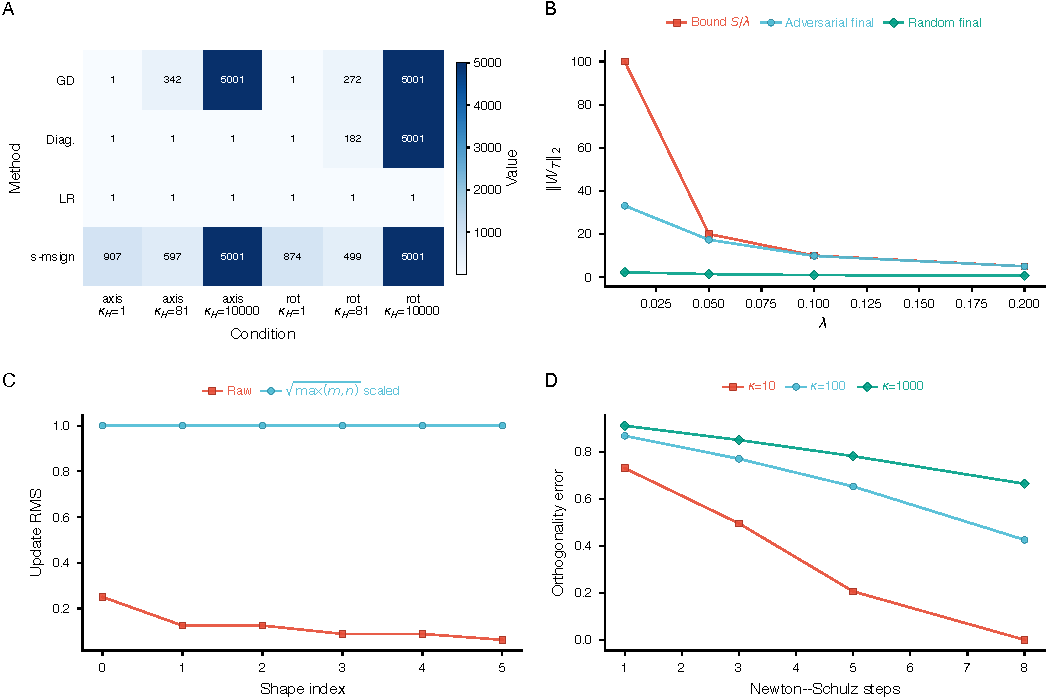
\includegraphics[width=0.98\textwidth]{figures/synthetic_diagnostics_composite.pdf}
    \caption{Synthetic mechanism diagnostics. (A) Matrix quadratics. (B) Decay control. (C) RMS alignment. (D) Newton--Schulz error.}
    \Description{Four-panel synthetic diagnostics for matrix quadratics, decay control, RMS alignment, and Newton--Schulz error.}
    \label{fig:synthetic_diagnostics}
\end{figure*}

Proposition~\ref{prop:decay} predicts that decoupled decay bounds the spectral norm of the weights when the update direction has bounded spectral norm. Proposition~\ref{prop:rms} predicts that the raw matrix-sign RMS scales as $1/\sqrt{\max(m,n)}$ for full-rank matrices. Tables~\ref{tab:decay_small} and~\ref{tab:rms_small} report the corresponding checks. The RMS table is a numerical SVD sanity check. It forms Gaussian matrices, computes the exact polar factor, and compares the observed RMS with the algebraic prediction. Figure~\ref{fig:synthetic_diagnostics}B--C shows the same conclusions visually. Adversarial polar updates approach but do not exceed the theoretical decay radius, and shape scaling restores unit RMS across matrix shapes.

\subsection{Newton--Schulz approximation quality}\label{sec:ns_exp}
We compare finite Newton--Schulz approximations with the exact SVD polar factor. Matrices are $32\times32$ with prescribed condition number. Alignment is the Frobenius cosine with the exact polar factor, orthogonality error is $\|X^\top X-I\|_F/\sqrt{n}$, and singular-value spread measures the remaining variation in the approximate polar factor. Table~\ref{tab:ns_small} and Figure~\ref{fig:synthetic_diagnostics}D show that additional steps improve alignment and orthogonality, whereas ill-conditioned matrices require more iterations. The experiment uses the standard cubic Newton--Schulz iteration. Optimization of polynomial coefficients is left to future work.

\begin{table}[t]
    \centering
    \caption{Weight-decay control under bounded spectral updates. Random and adversarial polar-update sequences are compared with the radius $S/\lambda$.}
    \label{tab:decay_small}
    \footnotesize
\begin{tabular}{lrrrr}
\toprule
$\lambda$ & Random max & Random final & Adv. final & Bound \\
\midrule
0.00 & 2.65 & 2.65 & 40.20 & inf \\
0.01 & 2.26 & 2.24 & 33.11 & 100.0 \\
0.05 & 1.42 & 1.39 & 17.33 & 20.0 \\
0.10 & 1.03 & 0.92 & 9.82 & 10.0 \\
0.20 & 0.73 & 0.65 & \textbf{5.00} & \textbf{5.0} \\
\bottomrule
\end{tabular}

\end{table}

\begin{table}[t]
    \centering
    \caption{Numerical SVD check of RMS alignment across matrix shapes. Exact-polar matrix-sign updates follow the $1/\sqrt{\max(m,n)}$ scaling for full-rank matrices.}
    \label{tab:rms_small}
    \footnotesize
\begin{tabular}{lcccc}
\toprule
Shape & Obs. RMS & Theory & Max error & Scaled RMS \\
\midrule
16x16 & 0.2500 & 0.2500 & 2.8e-17 & \textbf{1.00} \\
16x64 & 0.1250 & 0.1250 & 5.6e-17 & \textbf{1.00} \\
64x16 & 0.1250 & 0.1250 & 2.8e-17 & \textbf{1.00} \\
32x128 & 0.0884 & 0.0884 & 0.0e+00 & \textbf{1.00} \\
128x32 & 0.0884 & 0.0884 & 0.0e+00 & \textbf{1.00} \\
64x256 & 0.0625 & 0.0625 & 1.4e-17 & \textbf{1.00} \\
\bottomrule
\end{tabular}

\end{table}

\begin{table}[t]
    \centering
    \caption{Newton--Schulz approximation diagnostics. Alignment, orthogonality error, and singular-value spread are reported for each condition-number block.}
    \label{tab:ns_small}
    \footnotesize
\begin{tabular}{rrrrr}
\toprule
$\kappa(M)$ & Steps & Align. & Orth. err. & SV spread \\
\midrule
10 & 1 & 0.879 & 0.731 & 0.851 \\
10 & 5 & 0.994 & 0.207 & 0.341 \\
10 & 8 & \textbf{1.000} & \textbf{0.001} & \textbf{0.002} \\
100 & 1 & 0.687 & 0.869 & 0.985 \\
100 & 5 & 0.860 & 0.653 & 0.924 \\
100 & 8 & \textbf{0.957} & \textbf{0.426} & \textbf{0.748} \\
1000 & 1 & 0.569 & 0.912 & 0.999 \\
1000 & 5 & 0.721 & 0.782 & 0.992 \\
1000 & 8 & \textbf{0.824} & \textbf{0.665} & \textbf{0.974} \\
\bottomrule
\end{tabular}

\end{table}

The decay diagnostic and RMS numerical check address complementary quantities. Decay controls the norm of the weights, whereas RMS scaling controls the norm of the update. A polar direction without decay can accumulate over many steps, while a decayed polar direction without shape scaling can still induce layer-dependent update RMS. For this reason, the MLP diagnostic separates Muon, MuonW, RMS-MuonW, and Cov-MuonW.

\subsection{Finite Newton--Schulz inside MLP training}\label{sec:finite_ns_training}
To connect the approximation diagnostic with an actual optimizer step, we also replace the exact SVD polar factor in a MuonW-style MLP run by a finite Newton--Schulz approximation. The protocol uses the same Digits MLP architecture, full-batch training, momentum coefficient, weight decay, base learning rate, and bias policy as fixed-protocol MuonW. The only changed variable is the number of cubic Newton--Schulz steps $K\in\{1,3,5,8\}$ used to approximate the polar direction at each layer update. Table~\ref{tab:finite_ns_training} reports final test accuracy, final training loss, mean update orthogonality error across layers and epochs, and CPU runtime per run.

\begin{table}[t]
    \centering
    \caption{Finite Newton--Schulz MuonW training diagnostic on the Digits MLP. Accuracy, orthogonality error, and runtime are averaged over five stratified splits.}
    \label{tab:finite_ns_training}
    \footnotesize
\begin{tabular}{rrrrr}
\toprule
$K$ & Test acc. (\%) & Train loss & Orth. error & Runtime (s) \\
\midrule
1 & 95.11 $\pm$ 0.72 & 0.1511 & 0.8786 & 0.2775 \\
3 & \textbf{95.17} $\pm$ 0.72 & \textbf{0.1488} & 0.7046 & 0.3588 \\
5 & 95.06 $\pm$ 0.59 & 0.1491 & 0.5633 & \textbf{0.2613} \\
8 & 95.11 $\pm$ 0.57 & 0.1553 & \textbf{0.4370} & 0.2832 \\
\bottomrule
\end{tabular}

\end{table}

Increasing $K$ monotonically improves the mean orthogonality of the approximate polar factors in this training loop, but it does not produce a statistically meaningful accuracy ordering on this small dataset. This supports the narrower interpretation that finite Newton--Schulz quality affects the geometry of Muon-style updates, while task accuracy also depends on step scale, stochasticity, architecture, and tuning. The finite-NS table complements the standalone approximation diagnostic rather than replacing large-scale runtime or accuracy benchmarks.

\subsection{Small-scale Digits sanity checks}
We use the Digits dataset from scikit-learn, which contains $1,797$ examples with $64$ features. Features are standardized using statistics fitted on the training split. Logistic regression uses full-batch softmax cross-entropy for $100$ iterations. The MLP uses architecture $64\to32\to10$ with ReLU activation and is trained for $30$ epochs. Tables~\ref{tab:digits_fixed_small}--\ref{tab:mlp_stability_small} report fixed-setting accuracy, validation-selected accuracy, learning-rate selection, and MLP stability. AdamW is the main decoupled-decay baseline and the closest diagonal analogue of MuonW.

In logistic regression, RMS-MuonW performs best under the fixed learning-rate setting, whereas unscaled Muon variants are more sensitive to the chosen step scale. This result should not be read as intrinsic optimizer superiority. It indicates that shape-dependent scaling can substantially change the effective elementwise step size. The validation-selected protocol repeats both tasks with train, validation, and test splits and method-specific learning-rate grids. In logistic regression, Muon and RMS-MuonW both reach $96.00\%$ test accuracy, but RMS-MuonW uses a much smaller selected learning rate. In the MLP, MuonW obtains the highest mean test accuracy ($96.56\%$), while Cov-MuonW obtains the most favorable logit control among the Muon-style variants. These results support the weaker conclusion that scale and stability choices materially affect Muon-style steps. They do not show that a particular variant should dominate after broader tuning or at larger scale.

\begin{table}[t]
    \centering
    \caption{Small-scale Digits sanity check with logistic regression under the fixed-setting protocol. Test accuracy is averaged over five stratified splits.}
    \label{tab:digits_fixed_small}
    \begin{tabular}{lc}
\toprule
Method & Test accuracy (\%) \\
\midrule
GD & $93.83 \pm 0.75$ \\
Adam & $95.17 \pm 0.76$ \\
AdamW & $95.17 \pm 0.76$ \\
Muon & $92.78 \pm 1.04$ \\
MuonW & $92.72 \pm 1.09$ \\
RMS-MuonW & $96.11 \pm 0.93$ \\
Cov-MuonW & $94.67 \pm 0.90$ \\
\bottomrule
\end{tabular}

\end{table}

\begin{table}[t]
    \centering
    \caption{Small-scale Digits sanity check with the MLP under the fixed-setting protocol. Test accuracy is averaged over five stratified splits.}
    \label{tab:mlp_fixed_small}
    \begin{tabular}{lc}
\toprule
Method & Test accuracy (\%) \\
\midrule
SGD & $62.56 \pm 4.72$ \\
Adam & $95.17 \pm 0.52$ \\
AdamW & $95.17 \pm 0.52$ \\
Muon & $94.67 \pm 0.59$ \\
MuonW & $94.94 \pm 0.92$ \\
RMS-MuonW & $95.72 \pm 0.48$ \\
Cov-MuonW & $95.67 \pm 1.17$ \\
\bottomrule
\end{tabular}

\end{table}

\begin{table}[t]
    \centering
    \caption{Validation-selected learning-rate sweep for the Digits sanity checks. Learning rates are selected on validation and evaluated on test.}
    \label{tab:classification_sweep_small}
    \setlength{\tabcolsep}{1.2pt}
    \scriptsize
    \footnotesize
\begin{tabular}{llrrrr}
\toprule
Task & Method & Val. acc. & Test acc. & $\Delta$ AdamW & LR \\
\midrule
LogReg & SGD & $94.56 \pm 0.84$ & $94.67 \pm 1.28$ & $-0.78$ & 0.2 \\
LogReg & Adam & $95.33 \pm 0.92$ & $95.33 \pm 0.89$ & $-0.11$ & 0.03 \\
LogReg & AdamW & $95.33 \pm 0.92$ & $95.44 \pm 0.94$ & $+0.00$ & 0.03 \\
LogReg & Muon & $95.89 \pm 0.92$ & $96.00 \pm 0.38$ & $+0.56$ & 1 \\
LogReg & MuonW & $95.61 \pm 0.75$ & $95.61 \pm 0.21$ & $+0.17$ & 1 \\
LogReg & RMS-MuonW & $96.22 \pm 0.69$ & $96.00 \pm 0.38$ & $+0.56$ & 0.005 \\
LogReg & Cov-MuonW & $95.06 \pm 0.81$ & $95.28 \pm 0.25$ & $-0.17$ & 1 \\
\midrule
MLP & SGD & $88.44 \pm 0.97$ & $90.22 \pm 1.22$ & $-5.72$ & 0.2 \\
MLP & Adam & $95.56 \pm 0.68$ & $95.94 \pm 0.78$ & $+0.00$ & 0.03 \\
MLP & AdamW & $95.56 \pm 0.68$ & $95.94 \pm 0.78$ & $+0.00$ & 0.03 \\
MLP & Muon & $95.72 \pm 0.84$ & $95.94 \pm 0.33$ & $+0.00$ & 3 \\
MLP & MuonW & $96.33 \pm 0.81$ & $96.56 \pm 0.22$ & $+0.61$ & 3 \\
MLP & RMS-MuonW & $95.33 \pm 0.57$ & $95.50 \pm 0.37$ & $-0.44$ & 0.01 \\
MLP & Cov-MuonW & $96.44 \pm 0.27$ & $96.17 \pm 0.54$ & $+0.22$ & 3 \\
\bottomrule
\end{tabular}

\end{table}

\begin{table}[t]
    \centering
    \caption{Small-scale MLP stability sanity check under the fixed-setting protocol. Max logit and weight spectral norms are reported.}
    \label{tab:mlp_stability_small}
    \footnotesize
\begin{tabular}{lrrr}
\toprule
Method & Max logit & $\|W_1\|_2$ & $\|W_2\|_2$ \\
\midrule
SGD & 7.43 & 1.64 & 1.42 \\
Adam & 23.18 & 3.28 & 2.11 \\
AdamW & 23.07 & 3.27 & 2.11 \\
Muon & 20.99 & 2.23 & 2.43 \\
MuonW & 13.79 & 1.79 & 2.04 \\
RMS-MuonW & 81.45 & 5.36 & 4.12 \\
Cov-MuonW & 10.33 & 1.99 & 2.33 \\
\bottomrule
\end{tabular}

\end{table}

\begin{figure*}[t]
    \centering
    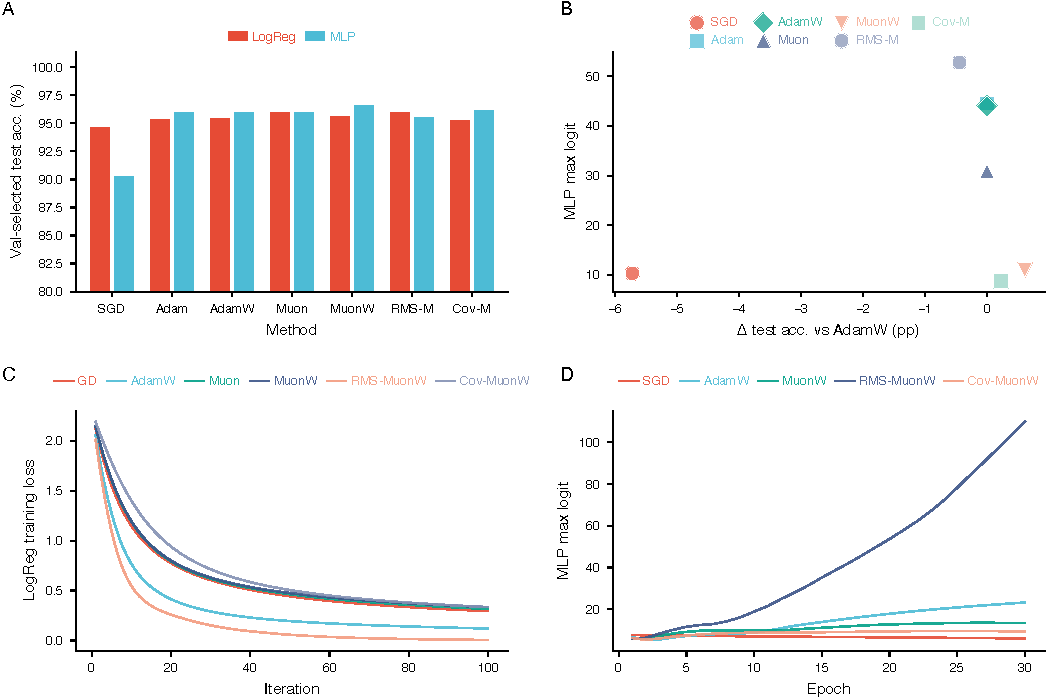
\includegraphics[width=0.98\textwidth]{figures/classification_diagnostics_composite.pdf}
    \caption{Small-scale Digits sanity checks. (A) Validation-selected test accuracy. (B) Accuracy gain versus MLP maximum logit. (C) Logistic-regression loss trajectories. (D) MLP maximum-logit trajectories.}
    \Description{Four-panel small-scale Digits sanity checks with accuracy, logit, and trajectory plots.}
    \label{fig:classification_diagnostics}
\end{figure*}

\section{Discussion and Limitations}
The analysis separates three mechanisms that are often conflated. Matrix preconditioning modifies the effective Hessian and can remove ill-conditioning on exactly solvable quadratics. The matrix-sign update modifies the singular values of the step and solves a spectral-norm constrained steepest-descent problem. Practical Muon-style training then depends on stability mechanisms. Decoupled weight decay controls weight growth. RMS alignment removes shape-dependent update scale. Newton--Schulz iterations approximate the polar factor efficiently.

\vpara{Scope of conclusions} The strongest conclusions are algebraic: the Kronecker Hessian, ideal left--right preconditioner, spectral-norm steepest-descent characterization, decay bound, RMS identity, and Newton--Schulz singular-value dynamics follow from the stated assumptions. The synthetic diagnostics support these mechanisms under controlled finite-dimensional settings. The finite-NS MLP diagnostic shows that approximation quality can be inserted into the training loop, but only in a small deterministic setting. The Digits sanity checks show that the same mechanisms leave measurable traces in accuracy, logits, and spectral norms on small full-batch classification tasks. Larger stochastic training settings are outside the scope of this course report.

\vpara{Implications} The diagnostics caution against treating Muon orthogonalization as a drop-in curvature preconditioner. On the quadratic model, a true left--right preconditioner removes the Hessian condition number, while the matrix sign changes the norm geometry of the update. On the Digits sanity checks, the validation-selected sweep shows that RMS scaling changes the effective step scale by construction, but its accuracy and stability effects depend on learning-rate selection. Decoupled decay, finite Newton--Schulz approximation, and covariance-assisted variants play different roles from the polar direction itself.

\vpara{Limitations} The experiments are low-dimensional, deterministic, and full-batch by construction. We do not evaluate language models, minibatch stochasticity, distributed communication, scalable runtime, or attention-specific mechanisms such as QK-Clip. The Cov-MuonW experiments use oracle full-batch covariances and exact SVD polar factors. They are covariance-preconditioned diagnostics and should not be treated as practical scalable baselines. The finite Newton--Schulz training diagnostic is included only for the small MLP and uses fixed hyperparameters. The Muon-family MLP bias policy is another confound: biases are updated by fixed-step gradient descent while Adam and AdamW update them adaptively. The scripts diagnose update geometry, not tuned benchmarks. The learning-rate sweep is intentionally small and should be read as a limited sensitivity check, not a full hyperparameter study. All experiment scripts set BLAS thread counts to one for reproducible CPU execution. The scaled matrix-sign update used in the experiments is also not identical to the fixed-radius spectral-norm step in Proposition~\ref{prop:msign}. The scaling improves numerical comparability, but it changes the step norm from $\eta$ to $\eta s_t$. Accordingly, the experiments evaluate the polar direction and its stabilizers rather than directly verifying the unscaled theorem.

\vpara{Future work} A larger empirical study would evaluate exact-polar, finite-Newton--Schulz, covariance-preconditioned, and RMS-scaled variants in Moonlight-style settings under validation-based tuning. Such a study should track weight RMS, update RMS, spectral norms, maximum logits, and wall-clock cost. It should also include minibatch stochasticity and larger matrix layers. A natural theoretical direction is to combine spectral-norm constrained updates with approximate curvature factors, thereby connecting Shampoo-style preconditioning with Muon-style orthogonalization.

\vpara{Code availability} Source code, experiment scripts, generated tables, raw CSV outputs, and the LaTeX source for this course report are publicly available at \url{https://github.com/Galaxy-Dawn/muon-optimization-course-report}.

\section{Conclusion}
Matrix preconditioning and Muon-style orthogonal updates address different mathematical objects. Full preconditioning can reduce the effective Hessian of a quadratic objective to the identity when the curvature factors are known. The matrix-sign update instead solves a spectral-norm steepest-descent problem and flattens update singular values. Decoupled weight decay, RMS alignment, and Newton--Schulz approximation are not merely implementation details. They are mechanisms that convert the spectral direction into a stable update rule. The controlled experiments support this separation. They also show that finite Newton--Schulz approximation quality changes update orthogonality and that apparent rankings in the Digits sanity checks are sensitive to step-size selection and stability scaling. These distinctions clarify both the potential and the limits of Muon-style optimizers as matrix-aware first-order methods.

\begin{acks}
This work was conducted as part of a graduate course on optimization.
\end{acks}

\bibliographystyle{ACM-Reference-Format}
\bibliography{references}

\appendix
\section{Reproducibility Statement}
The supplementary package contains scripts for all tables and figures, together with raw CSV outputs in the \texttt{results/} directory. The experiment README lists the exact commands. For reproducibility on CPU-only environments, the scripts set non-interactive plotting backends and use deterministic full-batch updates. Classification tables report five stratified splits. Feature standardization is fitted only on training data in both fixed-setting and validation-selected protocols. The validation-selected classification table is generated by the learning-rate sweep script in \texttt{experiments/}; table files are regenerated from CSV outputs by \texttt{write\_tables.py}.

\section{Optimizer Hyperparameters}
Table~\ref{tab:optimizer_hyperparams} lists the hyperparameters used by the fixed-protocol and validation-selected diagnostics. These values are included to make clear which quantities were tuned, which were fixed, and where implementation-level confounds enter the comparison.

\begin{table*}[t]
    \centering
    \caption{Optimizer and diagnostic hyperparameters. The grids are intentionally small diagnostic grids rather than exhaustive tuning ranges.}
    \label{tab:optimizer_hyperparams}
    \scriptsize
\setlength{\tabcolsep}{4pt}
\begin{tabular}{p{0.25\textwidth}p{0.68\textwidth}}
\toprule
Component & Hyperparameters \\
\midrule
Adam / AdamW & $\beta_1=0.9$, $\beta_2=0.999$, $\epsilon=10^{-8}$. AdamW applies decoupled weight decay $0.01$ to weight matrices. \\
Muon momentum & Exponential momentum coefficient $0.9$ for matrix gradients in Muon, MuonW, RMS-MuonW, Cov-MuonW, and finite-NS MuonW. \\
Covariance damping & Cov-MuonW uses oracle full-batch covariance inverses with damping $10^{-4}I$ before the exact SVD polar factor. This is a covariance-preconditioned diagnostic, not a finite Newton--Schulz implementation. \\
Fixed LogReg protocol & $100$ full-batch iterations. GD lr $0.1$; Adam/AdamW lr $0.01$; Muon/MuonW/Cov-MuonW base lr $0.1$ with gradient-norm scaling; RMS-MuonW lr $0.01$ with shape scaling. \\
Fixed MLP protocol & Architecture $64\to32\to10$, ReLU, $30$ full-batch epochs. SGD lr $0.05$; Adam/AdamW lr $0.01$; Muon lr $1.0$; MuonW lr $1.0$; RMS-MuonW lr $0.02$; Cov-MuonW lr $1.0$. \\
Finite-NS MLP protocol & Same MLP, splits, bias policy, momentum $0.9$, weight decay $0.01$, base lr $1.0$, and $30$ full-batch epochs as MuonW. The polar factor is approximated inside training by cubic Newton--Schulz steps $K\in\{1,3,5,8\}$ after Frobenius normalization; metrics report final test accuracy, train loss, mean layer-update orthogonality error, and wall-clock runtime per run. \\
Bias policy & For Muon-family MLP runs, matrix weights use the Muon-style update but biases use plain gradient descent with fixed bias lr $0.1$. Adam and AdamW update biases adaptively. This is an implementation-level confound for optimizer comparisons. \\
Validation LR grids & SGD: $\{0.02,0.05,0.1,0.2\}$; Adam/AdamW: $\{0.003,0.01,0.03\}$; Muon/MuonW/Cov-MuonW: $\{0.3,1,3\}$; RMS-MuonW: $\{0.005,0.01,0.02,0.05\}$. \\
Matrix quadratic protocol & Dimension $5\times5$, seed $0$, budget $5000$. GD and diagonal preconditioning use the minimax fixed step for the corresponding quadratic operator; LR uses $\eta=1$; scaled matrix sign uses base lr $0.02$. Convergence uses relative gap $f(W_t)/f(W_0)<10^{-8}$. \\
\bottomrule
\end{tabular}

\end{table*}

\section{Matrix-Quadratic Residual Diagnostics}
For the matrix-quadratic experiment, the stopping criterion is the relative objective gap $e_f=f(W_t)/f(W_0)<10^{-8}$. Table~\ref{tab:matrix_final_diag} reports both $e_f$ and the relative parameter error $e_W=\|W_t-W^\star\|_F/\|W^\star\|_F$ at termination or at the iteration budget.

\begin{table*}[t]
    \centering
    \caption{Final residual diagnostics for the matrix-quadratic experiment. Runs with $>5000$ did not meet the relative objective-gap tolerance within the budget or diverged numerically.}
    \label{tab:matrix_final_diag}
    \scriptsize
\setlength{\tabcolsep}{3pt}
\begin{tabular}{llrrrr}
\toprule
Rot. & Method & $\kappa$ & Iter. & $e_f$ & $e_W$ \\
\midrule
No & GD & 1 & 1 & $0$ & $0$ \\
No & Diag. & 1 & 1 & $0$ & $0$ \\
No & LR & 1 & 1 & $0$ & $0$ \\
No & s-\texttt{msign} & 1 & 907 & $9.9\times10^{-9}$ & $9.9\times10^{-5}$ \\
No & GD & 3 & 342 & $9.8\times10^{-9}$ & $4.6\times10^{-5}$ \\
No & Diag. & 3 & 1 & $1.5\times10^{-32}$ & $1.2\times10^{-16}$ \\
No & LR & 3 & 1 & $2.3\times10^{-32}$ & $1.2\times10^{-16}$ \\
No & s-\texttt{msign} & 3 & 597 & $9.8\times10^{-9}$ & $4.1\times10^{-4}$ \\
No & GD & 10 & $>5000$ & $6.9\times10^{-2}$ & $7.8\times10^{-2}$ \\
No & Diag. & 10 & 1 & $8.2\times10^{-33}$ & $1.3\times10^{-16}$ \\
No & LR & 10 & 1 & $1.2\times10^{-33}$ & $1.3\times10^{-16}$ \\
No & s-\texttt{msign} & 10 & $>5000$ & $2.5\times10^{202}$ & $9.9\times10^{100}$ \\
Yes & GD & 1 & 1 & $4.2\times10^{-31}$ & $6.1\times10^{-16}$ \\
Yes & Diag. & 1 & 1 & $4.3\times10^{-31}$ & $6.4\times10^{-16}$ \\
Yes & LR & 1 & 1 & $4.1\times10^{-32}$ & $1.4\times10^{-16}$ \\
Yes & s-\texttt{msign} & 1 & 874 & $9.8\times10^{-9}$ & $9.9\times10^{-5}$ \\
Yes & GD & 3 & 272 & $9.9\times10^{-9}$ & $9.1\times10^{-5}$ \\
Yes & Diag. & 3 & 182 & $9.9\times10^{-9}$ & $6.0\times10^{-5}$ \\
Yes & LR & 3 & 1 & $1.2\times10^{-31}$ & $4.5\times10^{-16}$ \\
Yes & s-\texttt{msign} & 3 & 499 & $9.9\times10^{-9}$ & $3.5\times10^{-4}$ \\
Yes & GD & 10 & $>5000$ & $4.3\times10^{-3}$ & $2.9\times10^{-2}$ \\
Yes & Diag. & 10 & $>5000$ & $7.9\times10^{-4}$ & $2.1\times10^{-2}$ \\
Yes & LR & 10 & 1 & $2.0\times10^{-30}$ & $1.2\times10^{-14}$ \\
Yes & s-\texttt{msign} & 10 & $>5000$ & $1.1\times10^{201}$ & $1.2\times10^{100}$ \\
\bottomrule
\end{tabular}

\end{table*}

\section{Use of Large Language Models}
Large language models were used for language editing and organization. The authors checked the mathematical derivations, code, and experimental results.

\end{document}
